\chapter{移动机器人的定位与导航}
\label{cha:chapter03}

定位与导航功能在机器人开发中占有重要地位。一般的,我们认为机器人的定位
导航功能包含环境地图构建、路径规划与运动控制以及自主避障等子任务。Tinker
机器人的定位导航系统基于ROS框架下的Navigation Stack实现,使用激光雷达、
里程计、深度相机等多传感器融合方法,能够完成实时地图构建、重定位、动态
环境下的避障即导航任务。


\section{SLAM方案的选择与性能分析}

Tinker最初使用的是建图与定位分开实现的方案。建图方面,我们使用
gmapping算法\cite{grisettiyz2005improving},
依赖2个北洋UTM-30LX单线激光雷达拼接定位(如图~\ref{fig:utm30lx})。定位
方面,我们使用基于蒙特卡罗的
amcl算法\cite{fox2002kld},两个算法同时工作时的可视化信息如图~\ref{fig:gmapping_amcl}。
amcl需要在地图已经给出的情况下进行定位,在
真实赛场上,比赛场景多数情况下是确定的,因此这套方案还基本可用,Tinker团队
会在开赛前对赛场进行扫描,将地图场景保存起来,之后比赛过程中单纯使用amcl
进行定位。后期随着团队成员对这套定位算法越来越熟悉,我们会将场景内可能出现
在单线雷达视野内的一切固定障碍的尺寸量下来,使用绘图软件对地图进行重建,然后
使用amcl进行定位,可以拿到更好的定位效果。

\begin{figure}
  \centering
  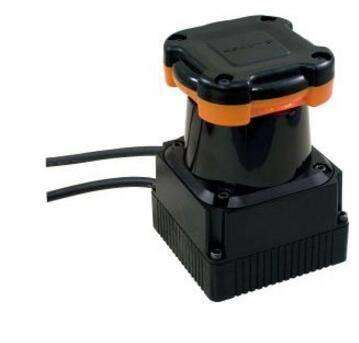
\includegraphics[width=150pt]{utm30lx.jpeg}
  \caption{北洋UTM-30LX单线激光雷达}
  \label{fig:utm30lx}
\end{figure}


\begin{figure}
  \centering
  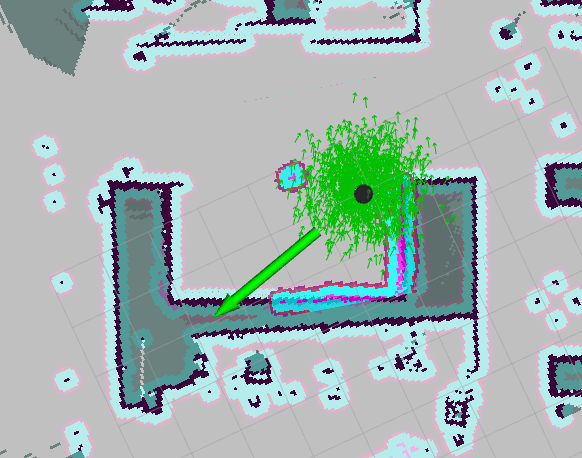
\includegraphics[width=300pt]{gmapping_amcl.png}
  \caption{Gmapping + Amcl可视化效果}
  \label{fig:gmapping_amcl}
\end{figure}

虽然上述方案在长时间内被证明是稳定可用的,但随着SLAM社区的不断发展,基于
粒子滤波的定位建图算法已经过时了,尤其是Google开源其自主开发的Cartographer
雷达建图定位算法\cite{hess2016real}之后,Tinker团队后期也将定位方案迁移为Cartographer+
ROS Navigation的模式,在更换建图定位算法之后,配合我们对Tinker硬件的二次
改版,我们也将原有的2个单线雷达减少为一个,变动之后定位数据减少,运算效率也
得到了提升。Cartographer的算法框架如图~\ref{fig:cartographer}所示。

\begin{figure}[h] % use float package if you want it here
  \centering
  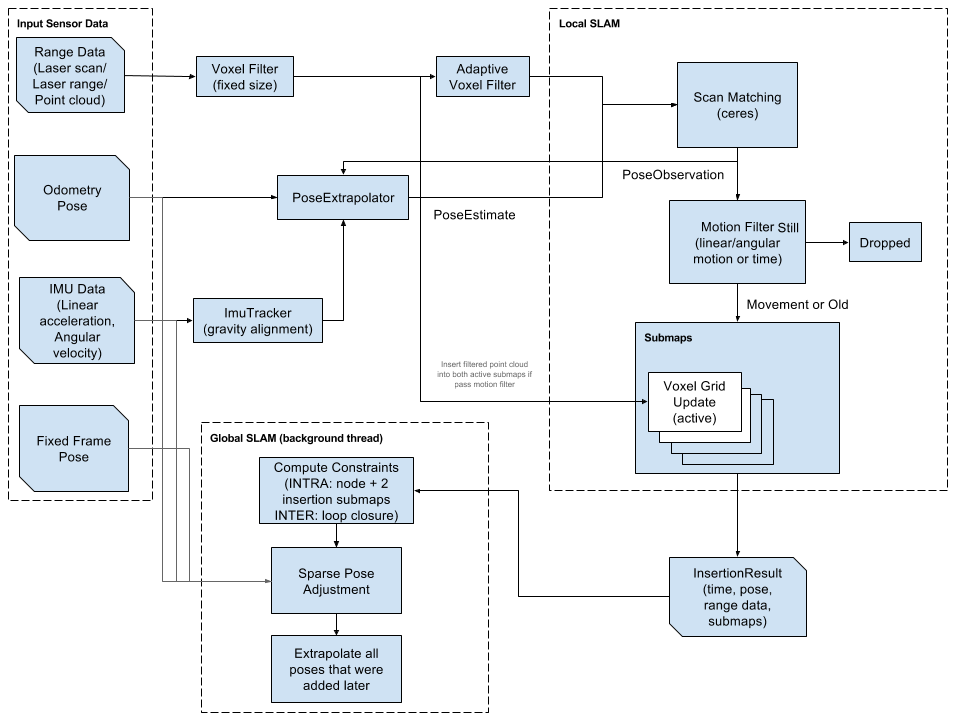
\includegraphics[width=.95\textwidth]{cartographer.png}
  \caption{Cartographer的算法框架}
  \label{fig:cartographer}
\end{figure}

除了基于单线激光雷达的各种定位建图算法外,笔者还尝试了一些基于特征点的视觉SLAM
方案,例如基于ORB特征点法的ORB-SLAM2(使用Kinect v2的RGB-D数据)\cite{mur2015orb},
ORB-SLAM2在室内环境中的可视化效果如图。。。所示。我们还测试了基于双目和IMU数据
融合的VINS-Fusion\cite{qin2018vins}算法,并且分析了两算法表现上的差异。

ORB-SLAM2的算法框架如图~\ref{fig:orb_frame}所示,其获取到原始数据后,首先对左右
目的图像提取特征,完成三角化,之后使用特征点的描述子在关键帧库中选取合适的帧
进行匹配,ORB-SLAM的关键帧选取策略较复杂,是一种基于共视关系的选取方案,即我们
在仓库中选取可能和当前帧看到同一场景的帧来进行匹配,在完成局部位姿优化后,经过
关键帧筛选策略选取关键帧,之后后端不断尝试通过词袋法发现相同场景,完成大的闭环
优化。VINS的算法框架如图~\ref{fig:vins_frame}所示,vins也是基于关键点法进行位姿
匹配的算法,同ORB-SLAM的主要区别有两个:一是VINS有IMU融合,其处理IMU数据的方式
为IMU预积分(IMU preintegration)\cite{forster2015manifold},且它将处理结果作为
优化项中的一个因子参与了位姿优化;二是VINS的
关键帧选择策略是简单的Sliding Window算法,即选取与当前帧在时间上相邻的几个关键帧
进行特征匹配与优化,这个策略和ORB-SLAM的共视图策略想比较略显粗糙,但是在大场景
下还是有不错的匹配效果。


\begin{figure}[h] % use float package if you want it here
  \centering
  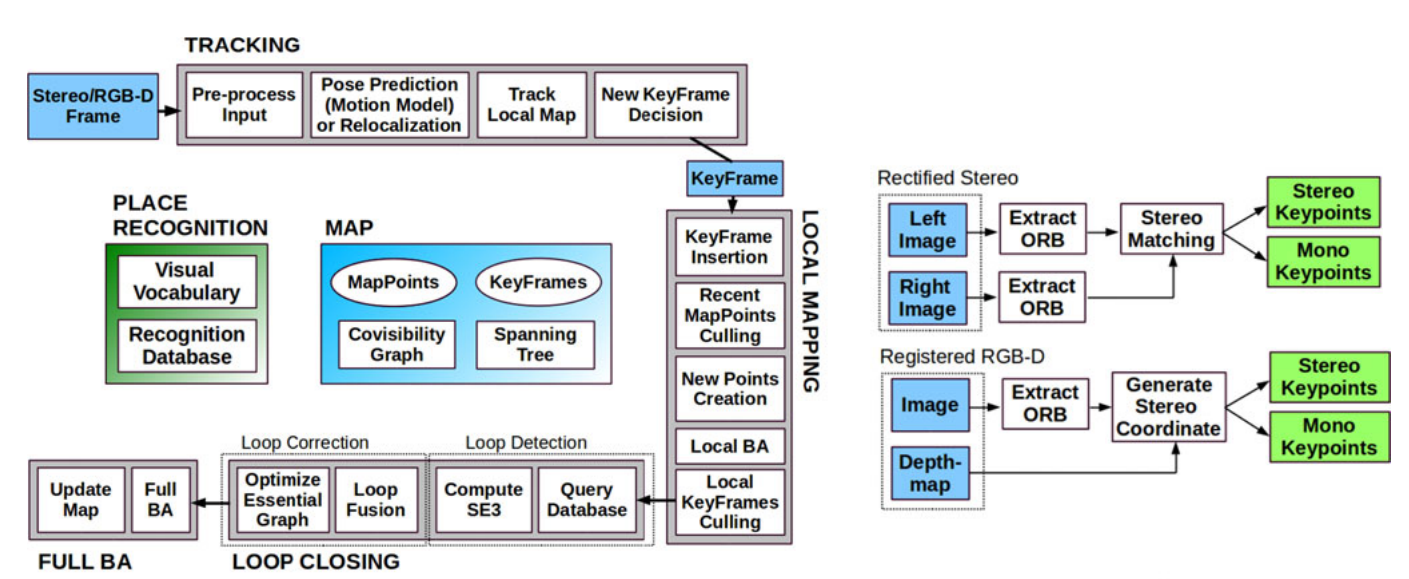
\includegraphics[width=.95\textwidth]{orb_framework.png}
  \caption{ORB-SLAM2的算法框架}
  \label{fig:orb_frame}
\end{figure}


\begin{figure}[h] % use float package if you want it here
  \centering
  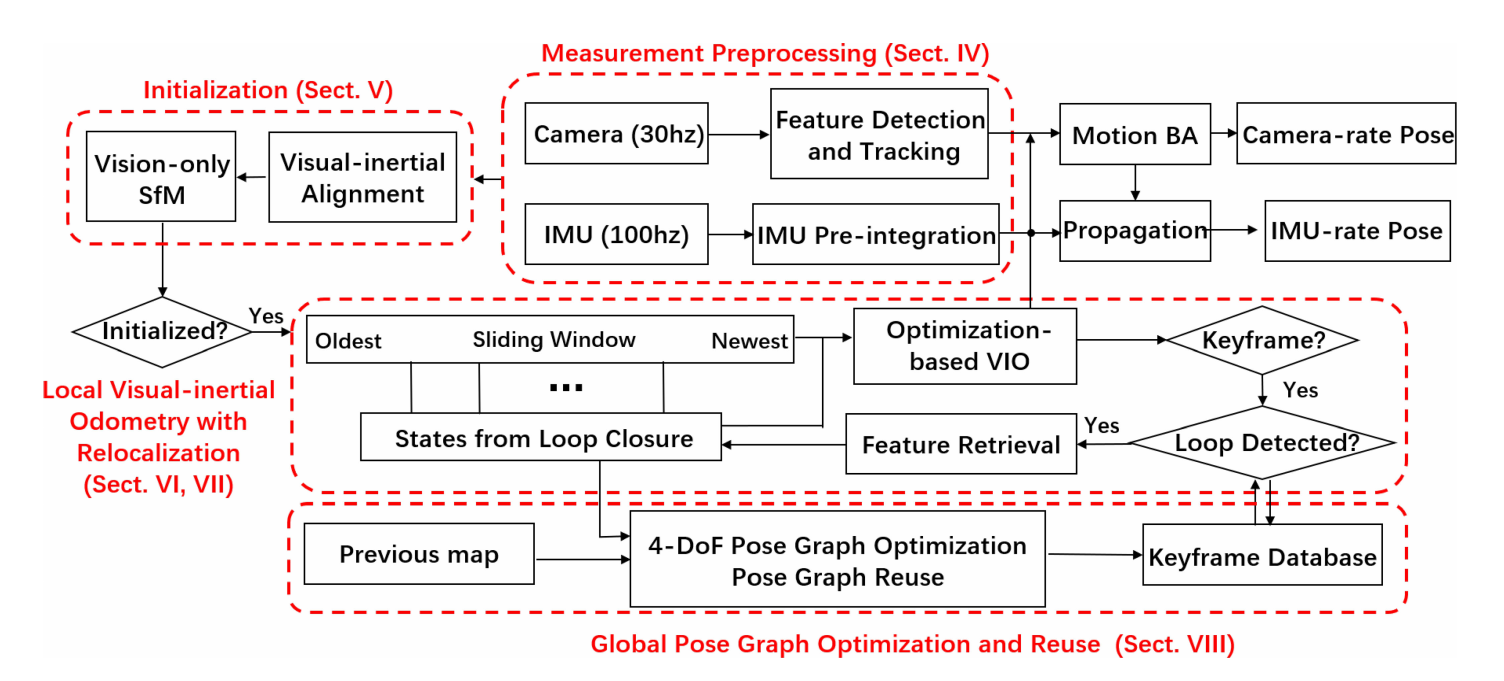
\includegraphics[width=.95\textwidth]{vins_framework.png}
  \caption{VINS-Mono的算法框架}
  \label{fig:vins_frame}
\end{figure}

\section{导航方案的选择}

Tinker的开发过程中一直使用ROS作为主要开发框架,而ROS的Navigation Stack中对于
导航避障提供了一套较为成熟的解决方案。Tinker前后使用了2套定位与规划算法,下面两个
章节中将对这两套方案进行详细描述。

\subsection{路径规划}

ROS的Navigation stack中提供了一整套导航避障的解决方案。其核心是同时维护地图信息
与路径规划器。地图信息使用一种分层管理的方式\cite{lu2014layered},并且分别维护
全局地图 Global Map与局部地图 Local Map。规划器也有两个,分别是Global Planner
和Local Planner。其中 Global Planner负责根据全局地图生成路径,而 Local Planner
则负责根据局部地图生成速度指令,传输给底盘执行。Tinker使用的 Global Planner是
一种基于 Dijkstra算法\cite{deng2012fuzzy}的路径生成方法,Local Planner是
一种基于dynamic window approach的速度生成方案\cite{fox1997dynamic}如图,其算法思想
为:在当前位置向各个方向以不同速度发射模拟路径,并且按照这些路径是否经过障碍物、
离目标路径的远近等等条件本别进行打分,选取分数最高的路径对应的速度极为dwa的输出
结果~\ref{fig:dwa}。上述
方案均为机器人导航领域较为经典且通用的方案,Tinker团队对上述算法进行了一些微调,以
使算法在Tinker平台上有更好的表现,如图~\ref{nav_costmap}所示为Tinker进行导航任
务时可视化的调试信息。


\begin{figure}[h] % use float package if you want it here
  \centering
  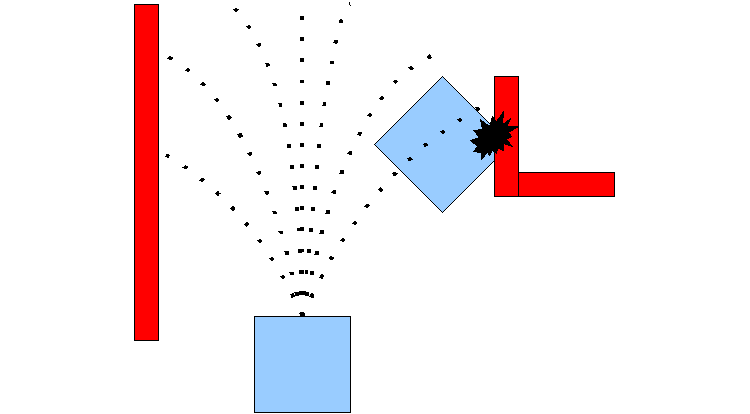
\includegraphics[width=1.\textwidth]{dwa.png}
  \caption{dwa算法示意图}
  \label{fig:dwa}
\end{figure}


\begin{figure}[h] % use float package if you want it here
  \centering
  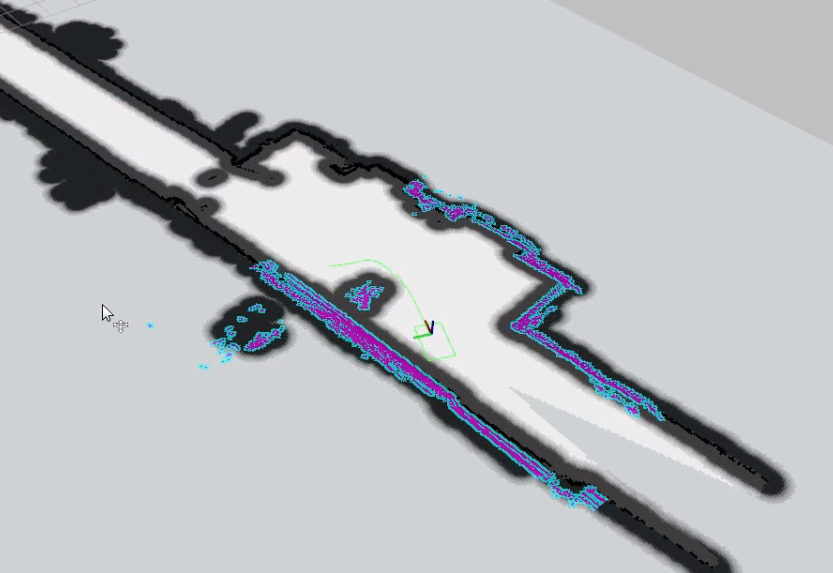
\includegraphics[width=1.\textwidth]{nav_costmap.png}
  \caption{进行导航任务时的地图与路径}
  \label{fig:nav_costmap}
\end{figure}

\subsection{机器人控制}

由于Tinker机器人使用全向麦克纳姆轮底盘,且每个电机控制一个麦轮,其运动学解算同
传统2轮底盘或者4轮阿克曼转向底盘相比更复杂一些。


\begin{figure}[h] % use float package if you want it here
  \centering
  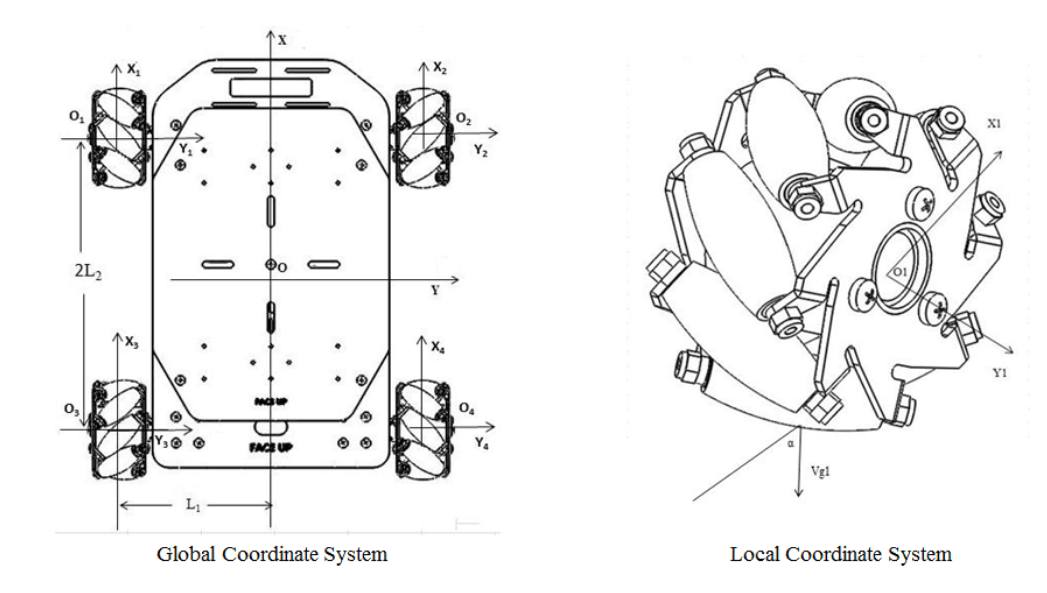
\includegraphics[width=.95\textwidth]{mecanum.png}
  \caption{麦轮底盘(左)与麦轮放大图(右),图片来源\cite{mecanum}}
  \label{fig:mecanum}
\end{figure}

如图~\ref{fig:mecanum}所示,假设底盘麦轮X型安装,其4轮到底盘中心的横向纵向距离分别
为$L_1$、$L_2$,四个车轮的转速为$\omega_1$、$\omega_2$、$\omega_3$、$\omega_4$
(即为电机转速),四个车轮上滚子的速度分别为$v_{g1}$、$v_{g2}$、$v_{g3}$、$v_{g4}$,
四个轮子的主轴的瞬时速度为$v_{O1x}, v_{O1y}$,$v_{O2x}, v_{O2y}$,$v_{O3x}, v_{O3y}$,
$v_{O4x}, v_{O4y}$,整个底盘的速度可表示为$v_x, v_y, \omega_O$,麦轮滚子轴与麦轮主轴
的夹角为$\alpha$(一般为\ang{45}),麦轮滚子轴到主轴的距离为$R$

根据速度分解,对1轮可列出~\ref{equ:glo_vec};对单个麦轮进行速度分析,可得~\ref{equ:loc_vec}

\begin{equation}
  \label{equ:glo_vec}
  \begin{aligned}
    v_{O1x} = v_x - \omega_O * L_1\\
    v_{O1y} = v_y - \omega_O * L_2
  \end{aligned}
\end{equation}

\begin{equation}
  \label{equ:loc_vec}
  \begin{aligned}
    v_{O1x} &= - v_{g1} * \cos\alpha + \omega_1 * R\\
    v_{O1y} &= v_{g1} * \sin\alpha
  \end{aligned}
\end{equation}

将~\ref{equ:glo_vec}~\ref{equ:loc_vec}两式联立消去轮速,可得~\ref{equ:mid_equ},
将两式合并消去$v_{g1}$,最终得到~\ref{equ:fin_equ}。

\begin{equation}
  \label{equ:mid_equ}
  \begin{aligned}
    v_x - \omega_O * L_1 &= - v_{g1} * \cos\alpha + \omega_1 * R \\
    v_y - \omega_O * L_2 &= v_{g1} * \sin\alpha
  \end{aligned}
\end{equation}


\begin{equation}
  \label{equ:fin_equ}
  \omega_1 = \frac{1}{R}
    \begin{bmatrix}
      1 & \frac{1}{\tan\alpha} & -(L_1 + \frac{L_2}{\tan\alpha})
    \end{bmatrix}
    \begin{bmatrix}
      v_x \\
      v_y \\
      \omega_O
    \end{bmatrix}
\end{equation}

因为此处$\alpha$取值为\ang{45},将其带入后可以得到四个轮子的电机输出转速与目标速度的转换
公式为\ref{equ:fin_all}

\begin{equation}
  \label{equ:fin_all}
  \begin{bmatrix}
    \omega_1 \\
    \omega_2 \\
    \omega_3 \\
    \omega_4
  \end{bmatrix}
    = \frac{1}{R}
  \begin{bmatrix}
    1 &  1 & -(L_1 + L_2) \\
    1 & -1 &  (L_1 + L_2) \\
    1 & -1 & -(L_1 + L_2) \\
    1 &  1 &  (L_1 + L_2) \\
  \end{bmatrix}
  \begin{bmatrix}
    v_x \\
    v_y \\
    \omega_O
  \end{bmatrix}
\end{equation}

值得一提的是,Tinker团队不断探索发现,在底盘接受速度命令端加一个smoother,对临近的
几帧速度命令进行一定程度的加权平滑(即一个一阶低通滤波器)~\ref{equ:filter}能够使
机器人的运动性能得到质的提升。

\begin{equation}
  \label{equ:filter}
  v_{final} = 0.9 * v_{origin} + 0.1 * v_{cur}
\end{equation}

这一发现也提示我们,对于机器人这一复杂系统来说,提升整体性能的手段是多元的,在制
定方案时应勇于尝试
多做实验,积极尝试各种想法,这样有助于我们使用较低的成本达到更好的性能。

